\graphicspath{{figures/}}
% Header
\renewcommand\evenpagerightmark{{\scshape\small Modeling metal organic frameworks}} 
\renewcommand\oddpageleftmark{{\scshape\small Chapter 2}}

%\renewcommand{\bibname}{References}

\hyphenation{}

\chapter[Modeling metal organic frameworks]%
{Modeling metal organic frameworks}
\label{ch2}
The understanding of catalytic processes in MOFs is a very challenging task. MOFs are materials of complex nature, and reactive processes in these materials are elusive and difficult to track on a purely experimental basis. Molecular simulations offer an alternative approach that starts from the construction of models that can explain, complement, and predict experiments. With growing computational power, computational models can aim at giving a more and more accurate description of materials at operating conditions, narrowing the gap between theory and experiment. Often, the structural properties and chemical transformations that take place on the active sites need to be investigated using a combination of multiple computational techniques, that allow to tackle the problem from different points of view. 
In this chapter, an overview of the different computational methods that can be used to study reactive processes in MOFs will be given. 
\td{check this part later}

\section{Framework topology}
A crucial decision when performing simulations lies in the choice of the model system, and what should be included in it. When choosing a model to represent the system under study, there is always a fine balance between accuracy and computational cost. 
On the one hand, it is crucial to use a computational model that captures all the relevant properties of the material and mimics the experimental structure as close as possible. On the other, it is often convenient to approximate and neglect certain properties in favor of a larger scale description of the processes. The focus in this work are the active sites that can be used for catalysis, therefore an accurate electronic description of this region of the material is imperative. Nevertheless, the activity of these sites for chemical reactions can also be influenced by other factors, such as the pore size or functionalization. Therefore, to describe active sites in MOFs and other nanoporous materials, which can have rather large unit cells and non-periodic structural defects, the first question that needs to be asked is how to account for periodicity. Two conceptually different approaches, which are described below, can be used.

\subsection*{Extended cluster model}
A very computationally efficient approach consists in neglecting periodicity and extracting a finite cluster of atoms from the periodic structure. This cluster model, displayed in Figure \ref{fig:clusterzoom}, contains the active sites and their surroundings but consists in a limited number of atoms, which decrease the computational cost. 
This allows both a more accurate treatment of the electronic structure, and a screening of different possible geometrical configurations of adsorbates, which is useful in the search for transition states. Moreover, very efficient transitions state searching algorithms have been developed for such systems in Gaussian, the most widely used code for cluster calculations.
When cutting a cluster, particular attention has to be drawn to the termination of bonds and the charge compensation, that have to be done in the most realistic way. The rest of the crystal structure does not surround the external cluster atoms. Some of these atoms need to be fixed in order to mimic the periodic environment and prevent nonphysical deformations that would affect an estimation of the entropy \cite{DeWispelaere2018}.

\begin{figure}[!htbp]
	\centering
 	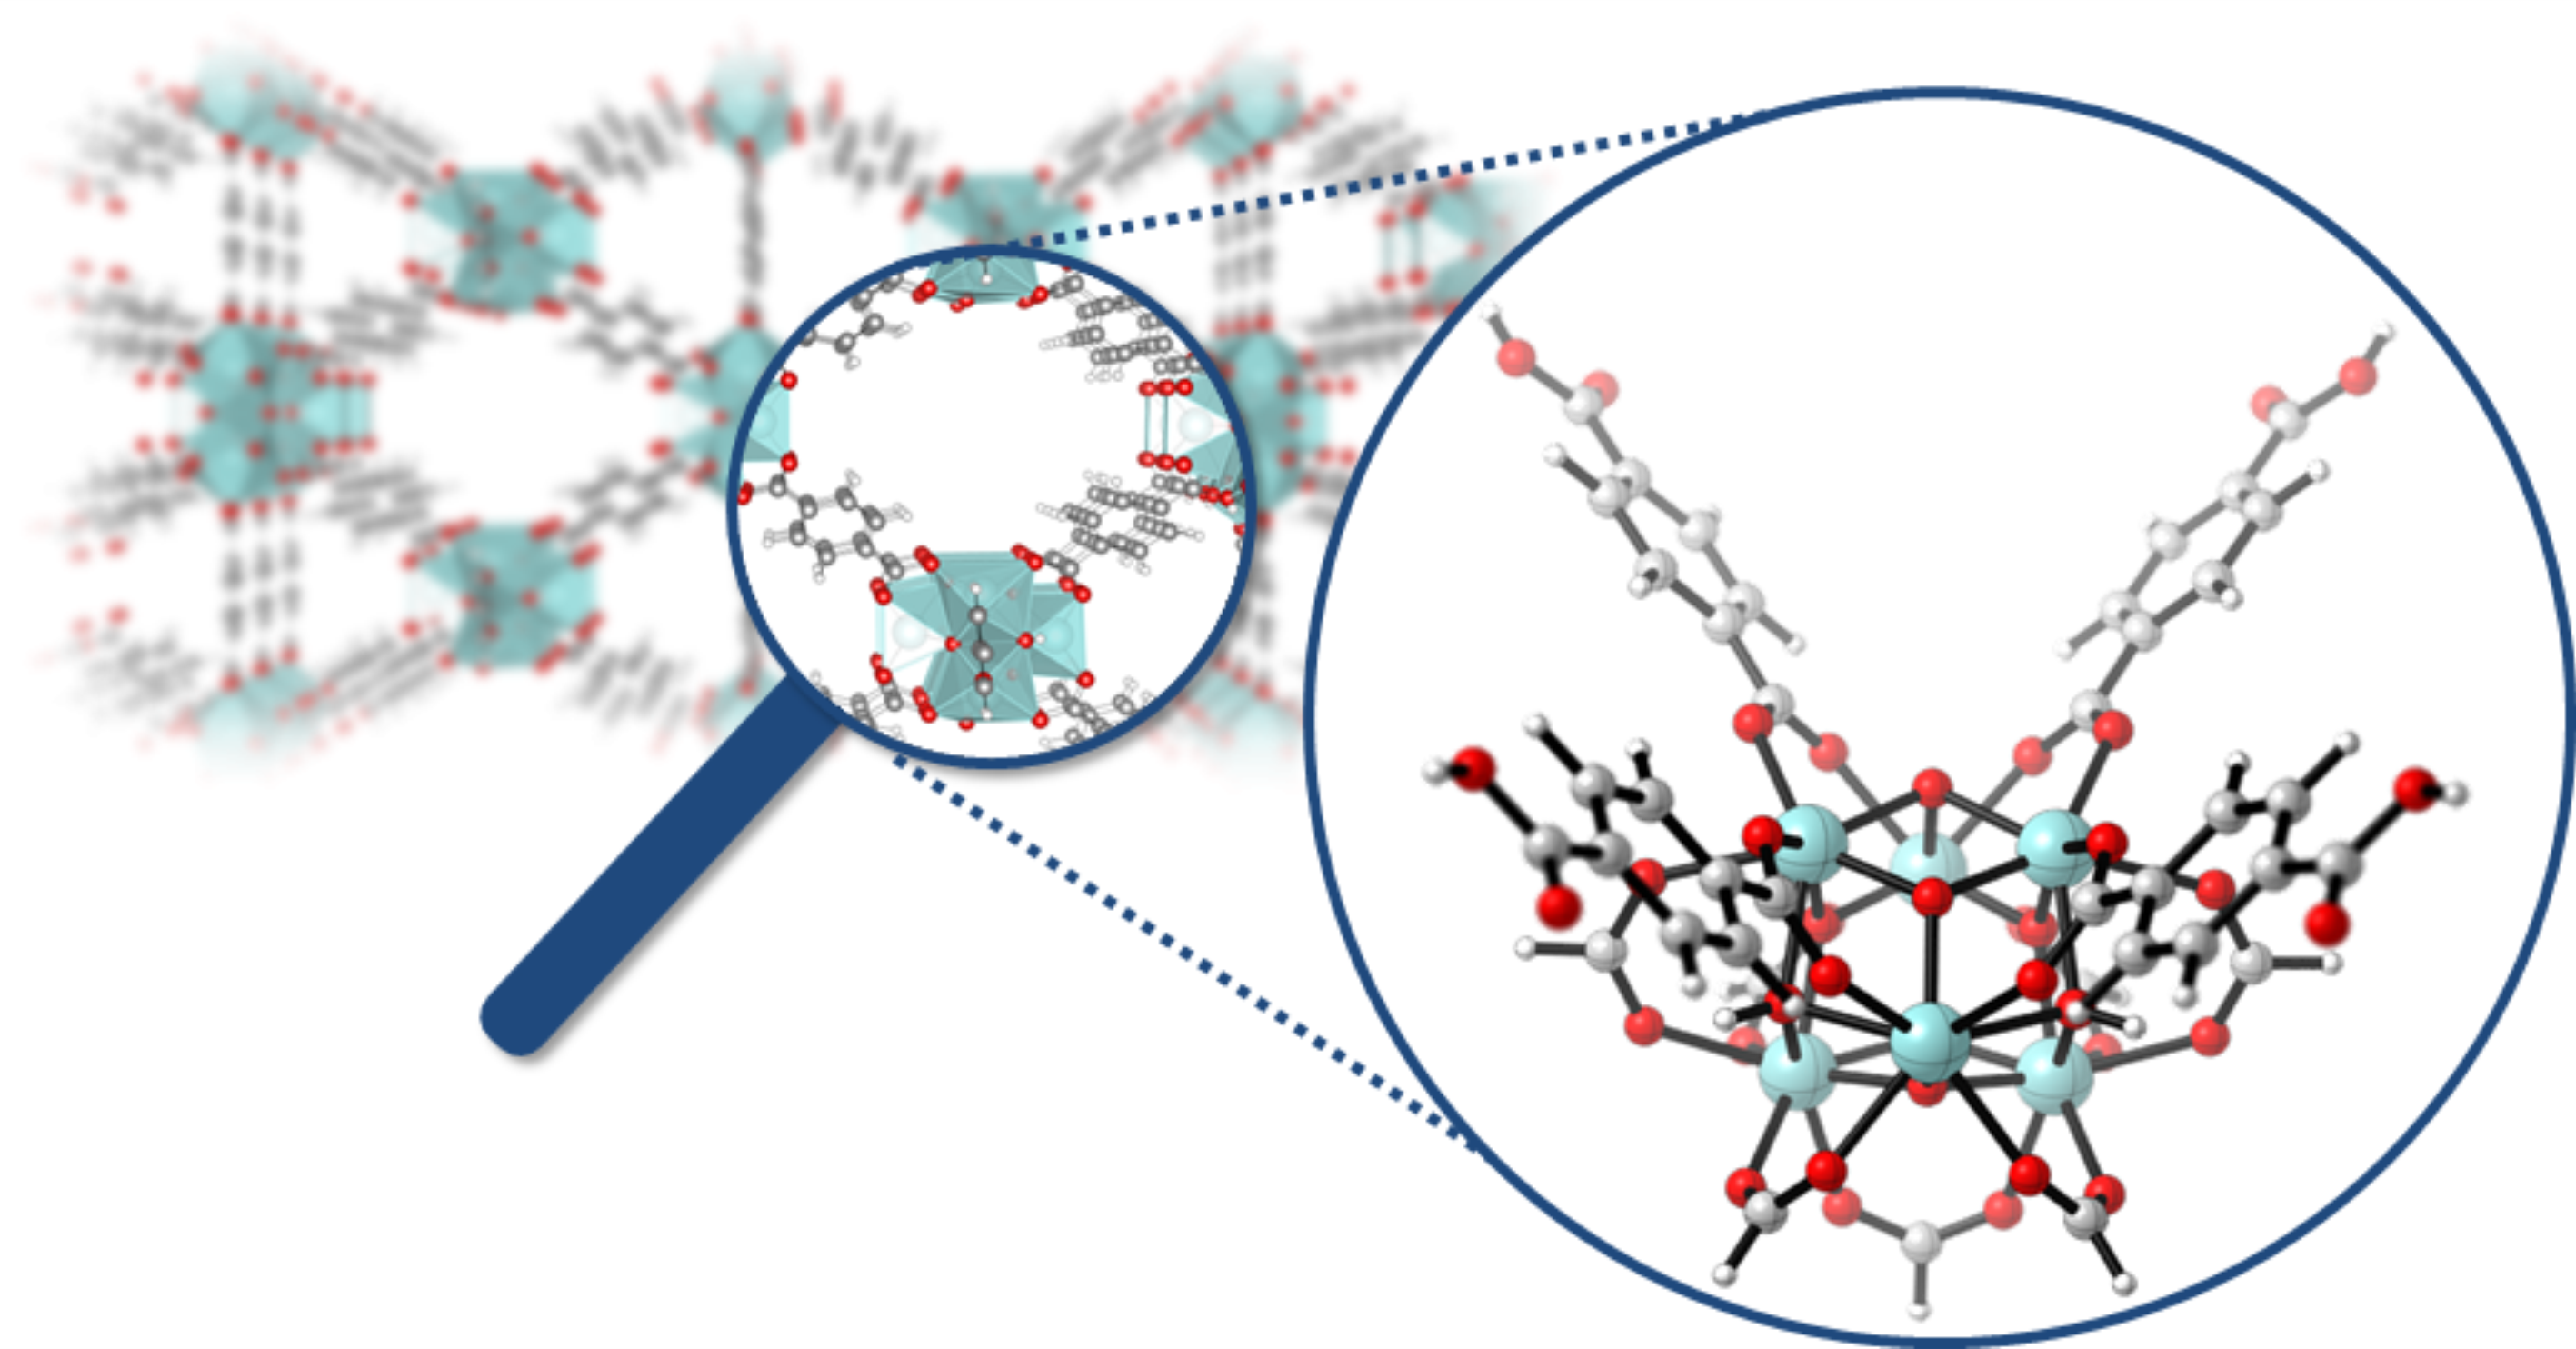
\includegraphics[width=1.0\textwidth]{clusterzoom}
	\caption{Extended cluster model cut from the periodic structure of UiO-66. The cluster contains the active site, the brick and the linkers in the closest proximity to the active site.}
	\label{fig:clusterzoom}
\end{figure}

Cluster calculations are an excellent way to benchmark and do a first qualitative screening of reactions and possible configurations and have been for long the standard computational tool when studying reaction in nanoporous materials. However, they are not adequate to correctly describe complex reactive processes, where confinement effect of the pores and structural rearrangements can play an important role. The role of solvent in the pores can also be crucial for the outcome of a reaction and cannot be explicitly studied by cluster models. Periodic calculations resolve this shortcoming, and as computational power grows, the heterogeneous catalysis community is shifting towards these more expensive, however more accurate models. 

\subsection*{Periodic model}
Periodic models enable to describe the whole topology of the framework. These calculations make use of periodic boundary conditions (PBC), which allow to simulate bulk phases with a limited number of atoms. In this model, the unit cell is replicated infinite times in each direction. When one atom disappears from one side of the unit cell it will reappear on the opposite side and each atom interacts with its neighbors in the same unit cell but also in the adjacent ones. Spurious interactions between the atoms can be avoided by applying a \textit{minimum image convention}, for which each atom interacts with its nearest neighbor or periodic image. In the case of long range interactions such as the electrostatic other techniques need to be used, such as Ewald summation \cite{Ewald1921}, where the potential is divided into a short range contribution, calculated in real space, and a long range contribution, calculated in reciprocal space using a Fourier transform. 
In the case of UiO-66, the conventional unit cell\cite{Cavka2008} contains 4 Zr bricks (Figure \ref{fig:periodic}, blue). In the calculations of this thesis, BDC linkers have been removed in the unit cell to introduce defects which are active sites in catalysis. Different amounts of missing linkers with different topologies have been considered. An interesting topology is the one denoted as type 6 in the work of Rogge et al.\cite{Rogge2017} that is characterized by a channel which offers good perspectives for the diffusion of guest molecules. This unit cell (displayed in blue in Figure \ref{fig:periodic}) can be reduced by symmetry to a 2-brick unit cell (in orange, Figure \ref{fig:periodic}) which offers the best compromise between accuracy and computational cost. This reduced unit cell is used in most of the calculations performed in this thesis.

\begin{figure}[!htbp]
	\centering
 	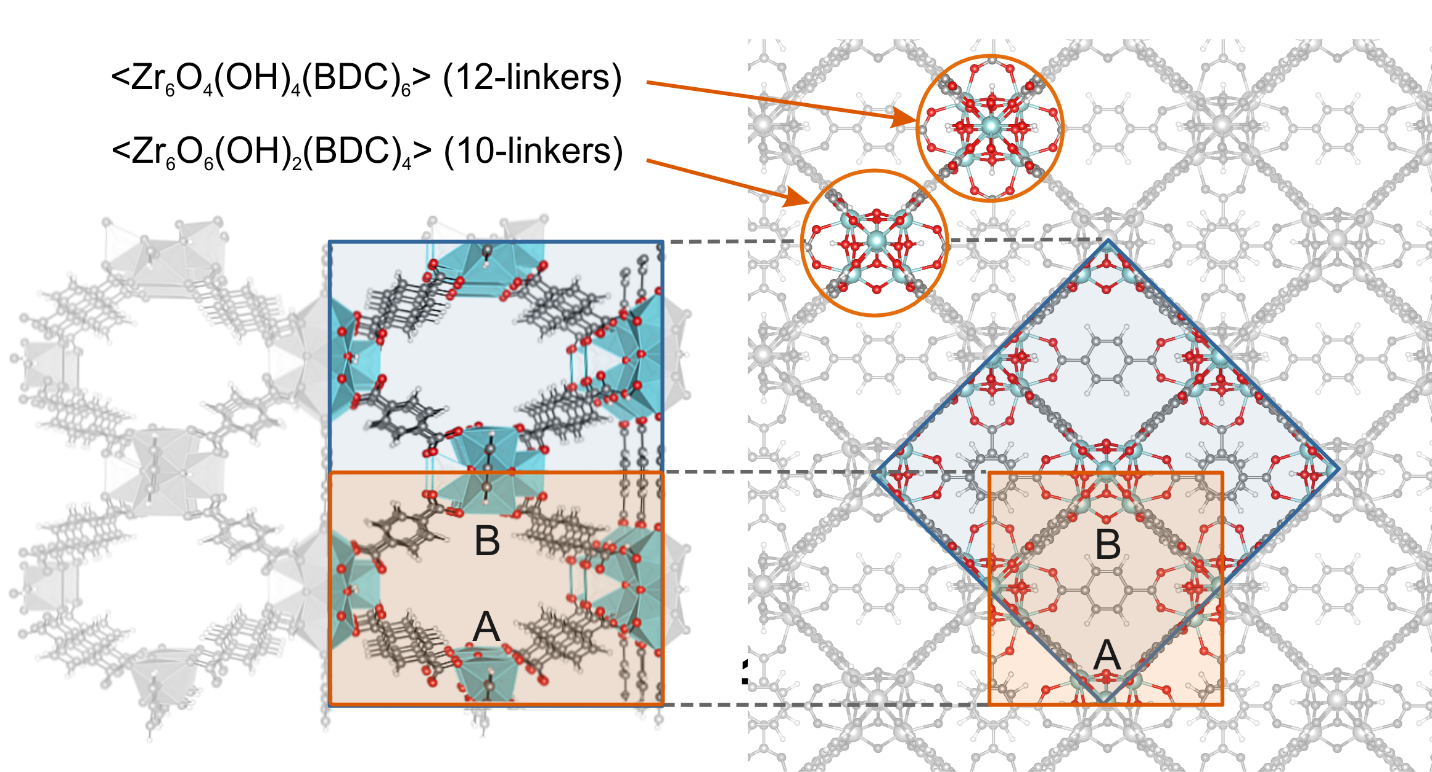
\includegraphics[width=1.0\textwidth]{periodic}
	\caption{Representation of the unit cells containing the defect. In blue, the conventional 4-brick unit cell, in orange, the 2-brick unit cell used for the calculations. The two different bricks are highlighted in orange. The 10-fold coordinated brick has two terephthalate linkers missing, one at site A and one at the opposite site B.}
	\label{fig:periodic}
\end{figure}

\section{Theoretical methods}
\subsection*{Electronic energy methods}
A basic quantity to study any chemical or physical transformation is the potential energy surface (PES), which is a function of the coordinates of all the atoms of the system. The PES is always the reference quantity in our simulations and every atomic configuration can be represented as a point in this hypersurface, with a given value of potential energy (Figure \ref{fig:BO-approx}).
Ideally, by calculating the value of the PES for each atomic configuration we can obtain all information on the system and on the transformations that can occur. However, the complexity of this surface escalates quickly with the number of atoms, and the sampling of its relevant regions represents the main challenge of molecular simulations. The information gained by exploring the PES is tightly connected to the experimental observables. Statistical physics acts like a bridge between the microscopic insight that is gained through molecular simulations and the macroscopic properties which are measured experimentally. In principle, all macroscopic properties of a system can be derived from its wavefunction. To calculate it, the stationary Schr\"{o}dinger equation is solved: 
\[
\hat{H}\left\vert\psi\right\rangle = E\left\vert\psi\right\rangle
\]

where $\psi$ is the wavefunction, $\hat{H}$ is the Hamiltonian of the system, and $E$ is the total energy. The resolution of this equation is at the heart of computational chemistry and will in principle provide the exact description of matter, but it is nevertheless extremely difficult to solve for most of the electron systems. The presence of electron--electron interactions makes it a highly coordinated problem, and for this reason, different approximations need to be applied, to remove the interactions that have a minimal contribution to the energy.

\subsection*{Born--Oppenheimer approximation}

\begin{figure}[!htbp]
	\centering
 	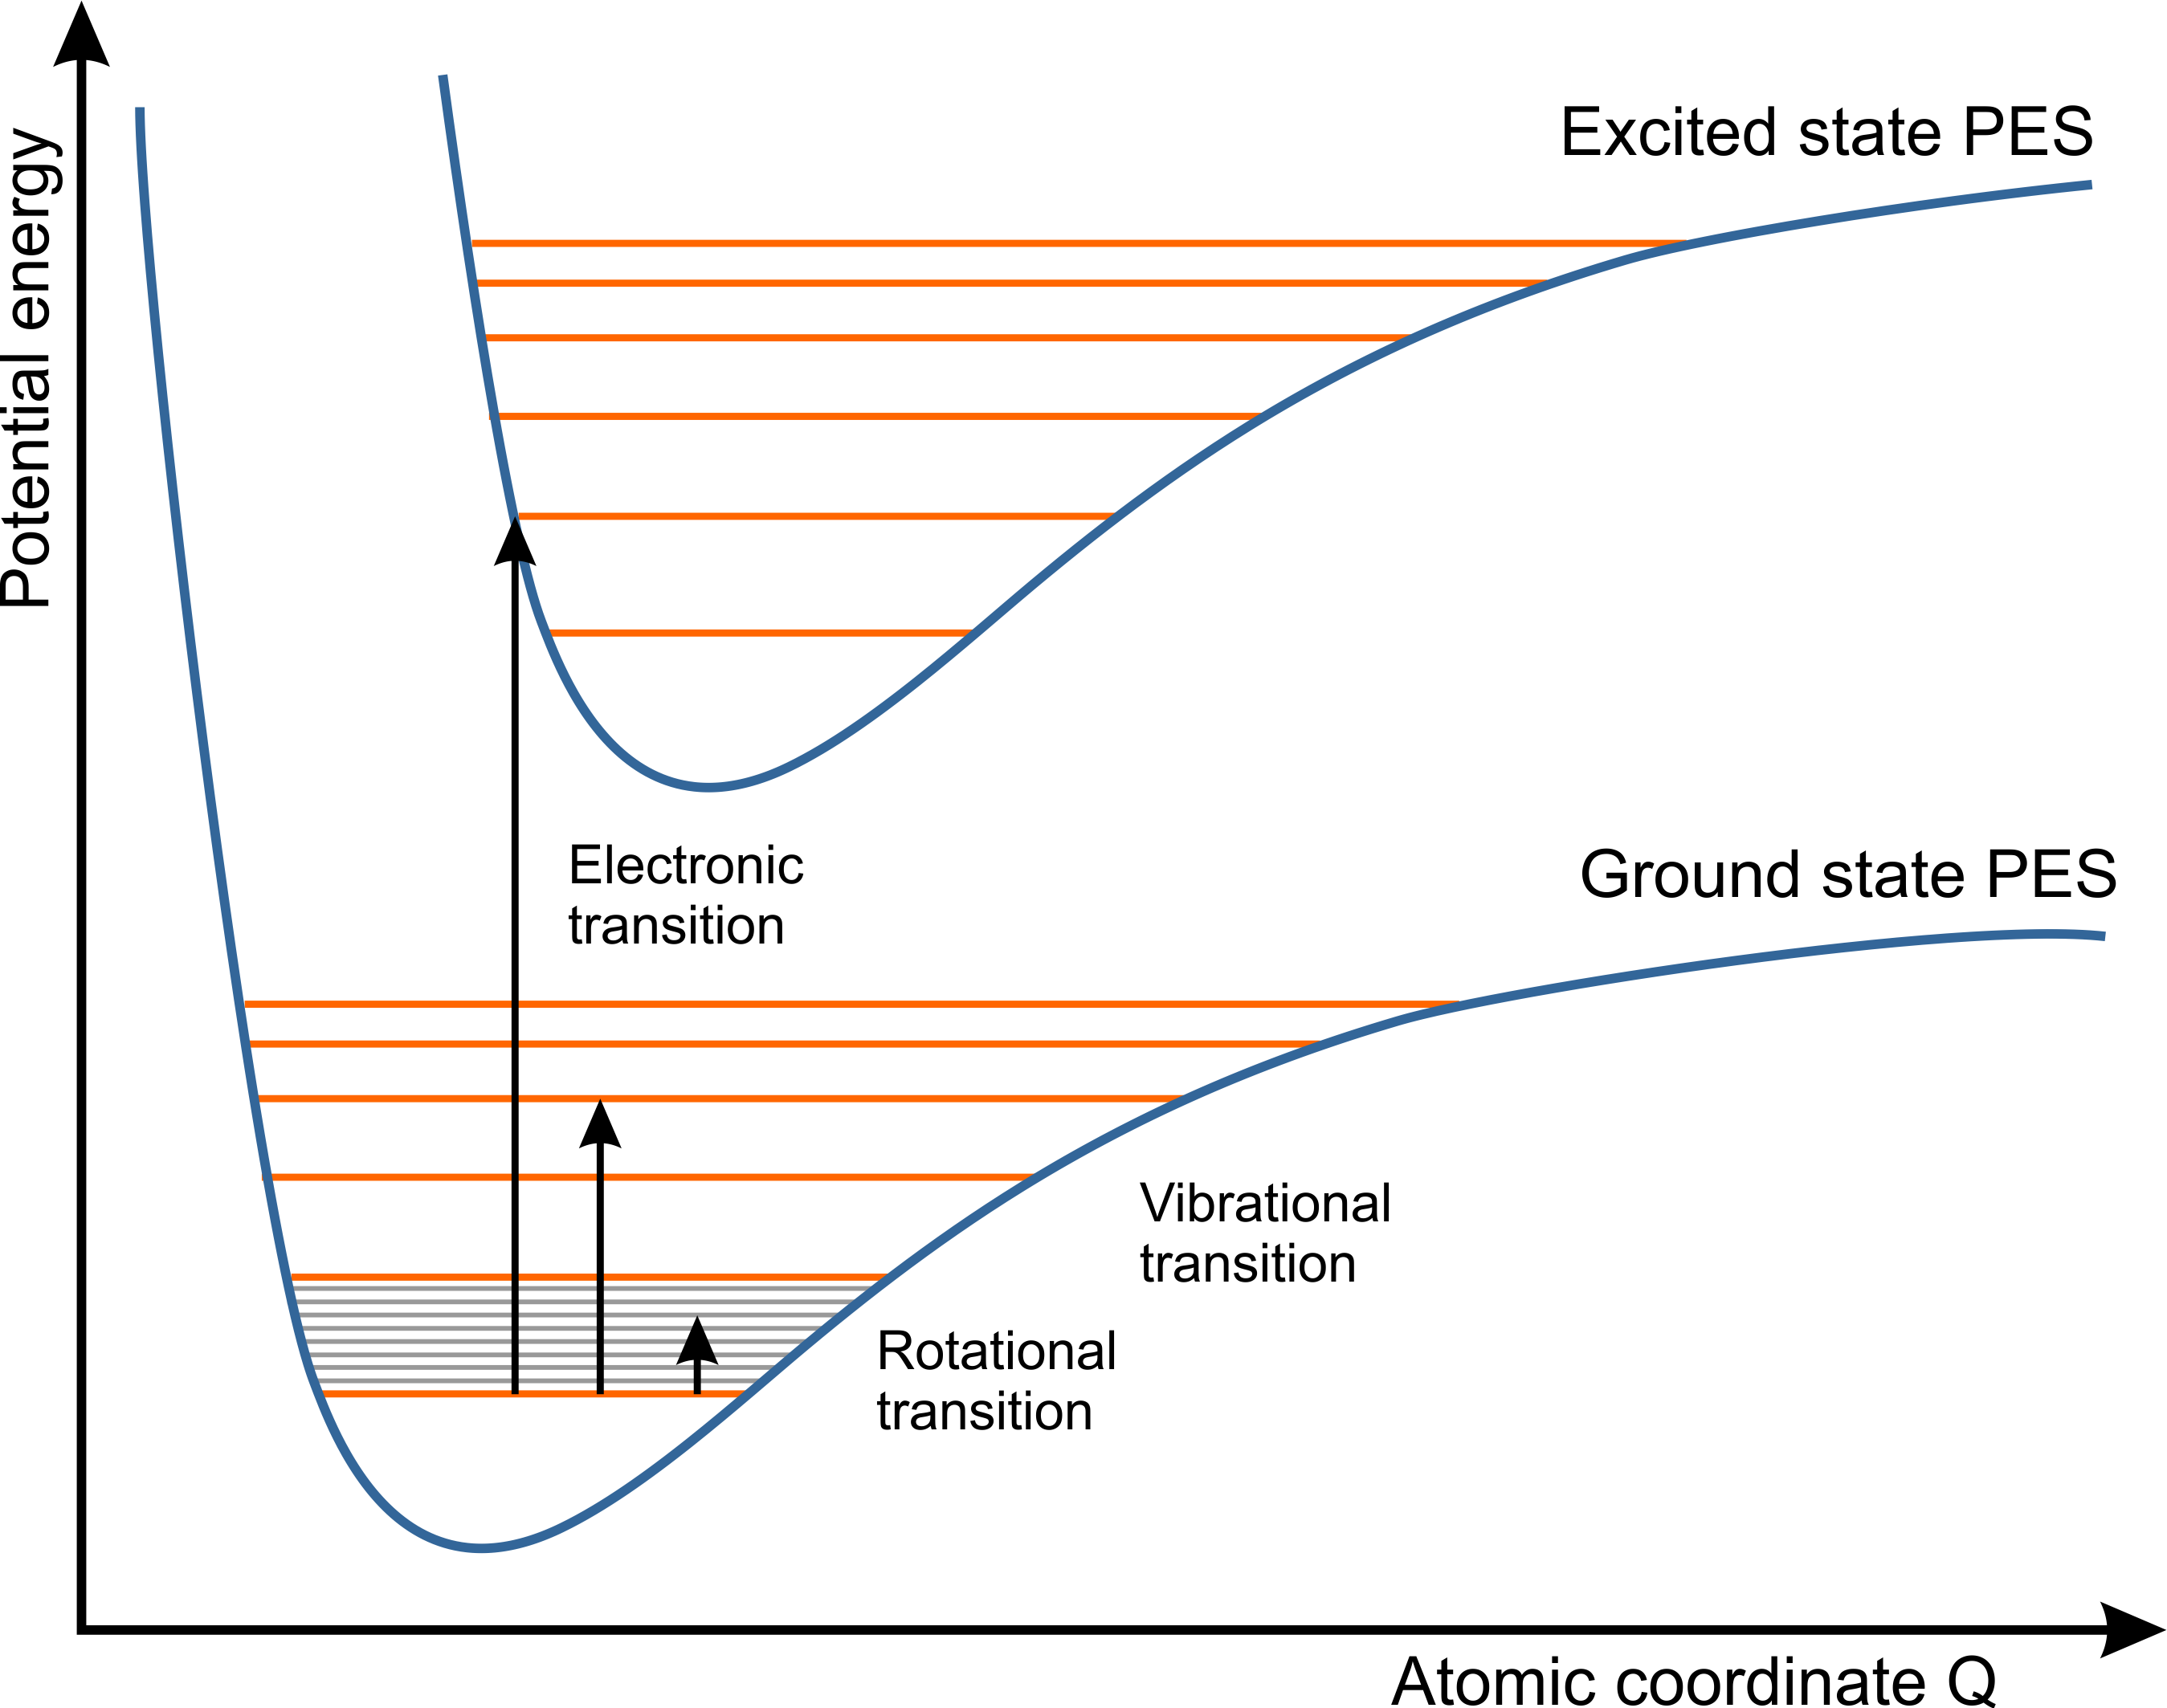
\includegraphics[width=1.0\textwidth]{BO-approx}
	\caption{The two lowest PES in the BO approximation for a diatomic molecule. In blue, the electronic PES for the ground state and first electronic excited state (UV-Vis transition). In orange, the vibrational energy levels (IR transitions), in grey the rotational levels (microwave transitions.}
	\label{fig:BO-approx}
\end{figure}

For all calculations performed in this work, we rely on the so-called Born-Oppenheimer (BO) approximation \cite{Born1927}. In this treatment, nuclei are considered as classical points which move in the potential energy surface generated by the electrons (Figure \ref{fig:BO-approx}). This way, to each nuclear configuration a corresponding electronic energy can be assigned, and nuclear coordinates enter in the Schr\''odinger equation only as parameters, allowing to construct a BO surface, or PES. This approximation holds since nuclei are much slower than electrons, therefore the motion of electron is instantaneous from the nuclei point of view. 
This approximation is not always possible, especially when dealing with light nuclei such as hydrogen. In these cases, nuclear quantum effects can have an impact on the measured properties \cite{Ceriotti2016}. In most cases, the electronic ground state is also not interacting with the higher electronic states because of the high energy difference. In the BO approximation, the electronic energy levels are also considered fully separated and do not interact with each other. For this reason, the approximation is also called adiabatic approximation. Additional interactions have to be considered when two surfaces lie close to each other, for instance in the neighborhood of conical intersections. 

\subsection*{Force Fields}

\begin{figure}[!htbp]
	\centering
 	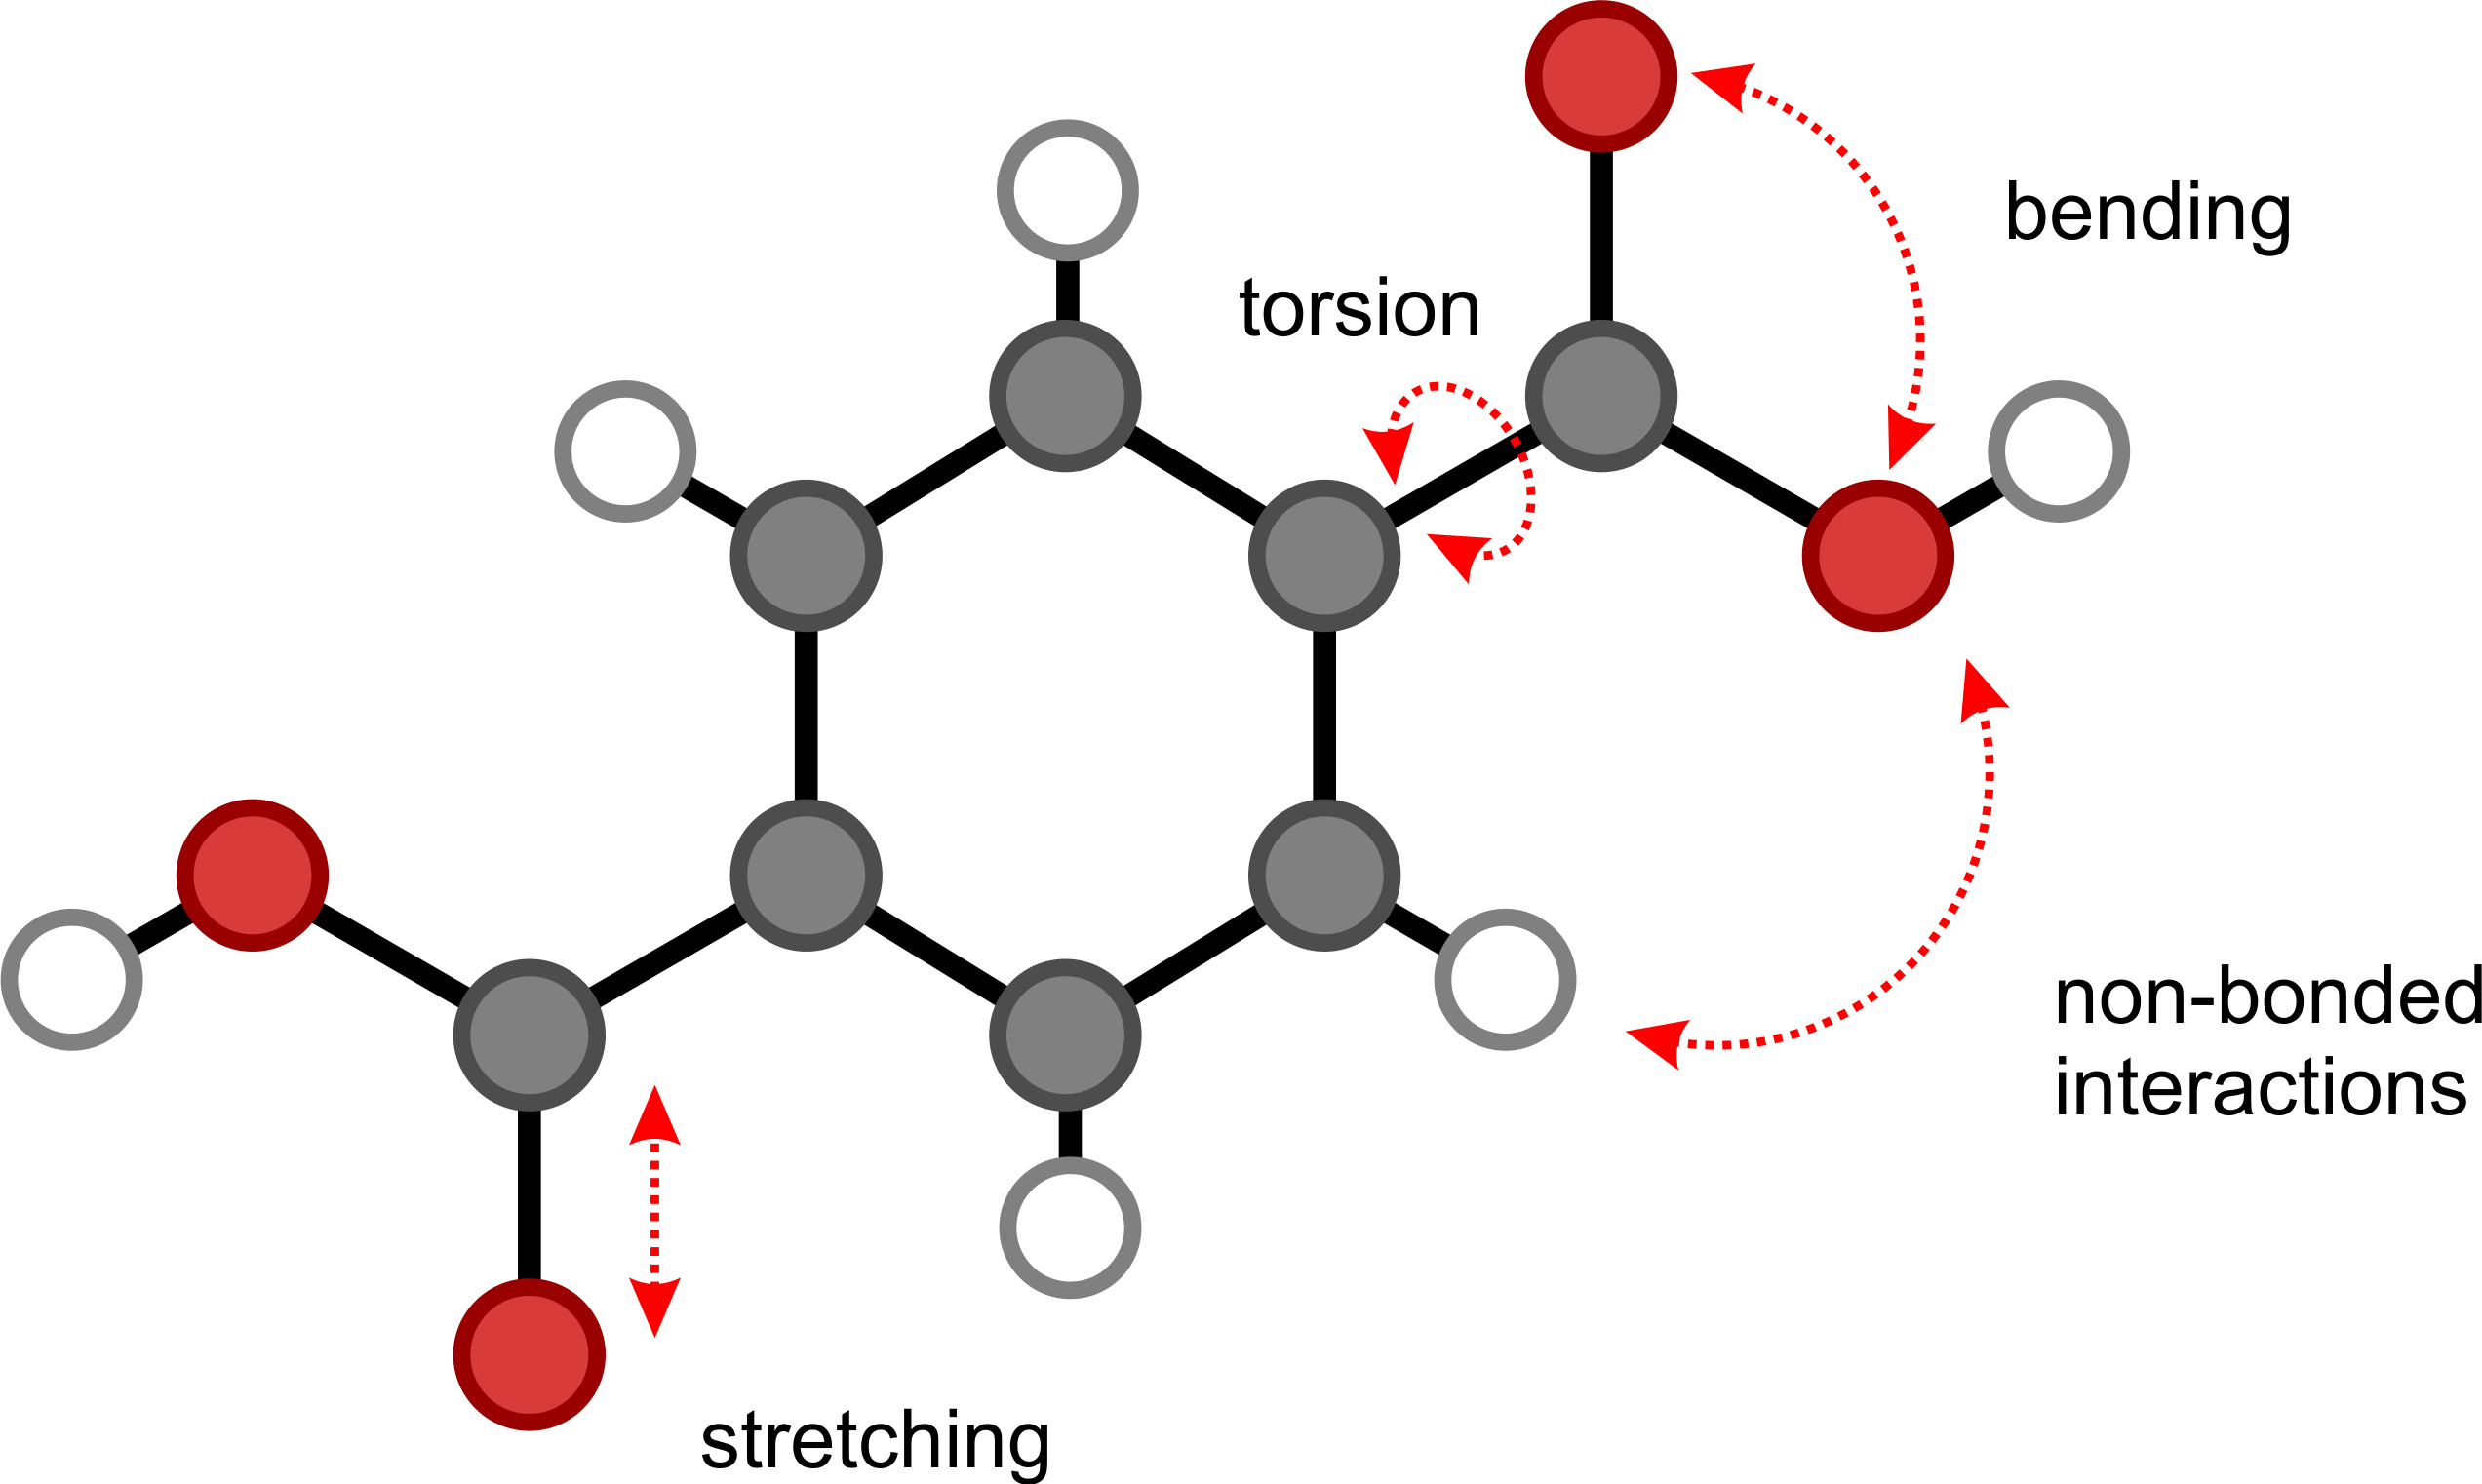
\includegraphics[width=1.0\textwidth]{forcefield}
	\caption{Representation of some of the molecular modes taken into account in a generic force field model.}
	\label{fig:forcefield}
\end{figure}

The simplest way to describe interactions between atoms which determine the PES is the so-called ``balls and springs'' model. In this treatment, all interactions are represented by interatomic classical potentials which are parametrized to reproduce the results of more accurate quantum mechanical calculations. In this work, generic force field calculations have been used in some cases to give preliminary input structures for more costly \textit{ab initio} calculations, through which the description of chemical transformations is possible. 
Force fields are often constituted by harmonic potentials which do not allow bonds being broken and formed (Figure \ref{fig:forcefield}). Reactive force fields, such as ReaxFF \cite{VanDuin2001} are currently being developed, but their application in complex heterogeneous reactions is still an ongoing chemical challenge and is out of the scope of this work. For this reason, the description of reactive processes needs a more advanced treatment, where electronic distributions are explicitly taken into account.

\subsection*{Density Functional Theory}
Density functional theory (DFT) has become the method of choice for the study of chemical systems, due to its good trade-off between computational cost and accuracy of the obtained results. DFT began in the 1920’s with the work of Thomas and Fermi  \cite{Thomas1927, Fermi1928}, but it was only in the ’60s that it became a complete and accurate theory, shown in the work of Kohn, Hohenberg and Sham\cite{Hohenberg1964}. The fundamental property that DFT describes is electron density as opposed to many body electron wavefunctions, which allows to reduce enormously the number of variables in the case of complex systems. Two fundamental theorems by Hohenberg and Kohn state that there is a unique relation between electronic density and total wavefunction, therefore the ground state density allows us to determine all properties of the system. Moreover, the ground state density can be obtained from a minimization of the total energy functional with a variational method by solving the so-called Kohn-Sham equations. The global minimum value of the functional determines the exact ground state of the system. This way it is possible to obtain the total energy of the system and the forces which act on the atoms, two quantities which are needed in all the simulations performed in this work. 

In principle, DFT is an exact method, but the minimization of energy is far from trivial. Kohn and Sham \cite{Kohn1965} introduced a method which replaces the many-body problem with an auxiliary system of non-interacting particles, allowing a fast solution of the eigenvalue problem. What needs to be added in this treatment is an additional functional which describes exchange and correlation. Nowadays one of the greatest challenges in DFT consists in the search for an accurate expression for the exchange-correlation functional.
 The simplest is known as Local Density Approximation (LDA) initially proposed by Kohn and Sham \cite{Kohn1965} and can also be adapted to include spin in the Local Spin Density Approximation (LSDA) \cite{Vosko1980}. A more refined method is the Generalized Gradient Approximation (GGA) which involves the calculation of the gradient of electron density and includes functionals such as B88 \cite{Becke1988}, LYP \cite{Lee1988} and PBE \cite{Perdew1996, Perdew1997}, used in this thesis. 
 More recent functionals are the so-called hybrid functionals, which include the Hartree-Fock (HF) exchange, such as B3LYP \cite{Becke1988, Becke1993, Lee1988}, which is a combination of B88, LYP and LDA with HF, and PBE0 \cite{Adamo1999}, which mixes PBE with HF. These functionals can give a more accurate electronic description of the system but are computationally very expensive. As compromise between accuracy and computational cost, what is often performed in the simulation of this thesis is a geometry optimization with PBE, and a single point calculation to refine the energies with B3LYP.

\subsubsection*{Dispersion interactions}
In this thesis we often encounter non-covalent interactions which need to be treated with high accuracy, such as the adsorption of guest molecules on the Zr Lewis acid sites or interaction between solvent molecules. One of the challenges of DFT methods is the description of long range dispersive interactions such as London forces, which are commonly referred to as van der Waals interactions. These interactions are due to many particle electron correlation effects which are present also in absence of charges and can have a significant impact on the non-covalent interaction energy. To tackle this problem, various dispersion schemes have been proposed. One of the most used is currently the Grimme--D3 method \cite{Grimme2010}, where a damped $-C_{6}R^{-6}$ function is added to the DFT functional. Recently, more advanced dispersion schemes have been developed, such as the many body dispersion scheme \cite{Buko2016}, or the one of Tkatchenko and collaborators \cite{Ambrosetti2014}, although for the systems we are studying not many benchmarks of these new methods have been performed so far  \cite{Wieme2018}.

\subsection*{Geometry optimization}
In order to obtain molecular structures that have physical significance and their relative energies, the arrangement of the atoms needs to be optimized. There are generally two types of molecular structures that we need to find in our simulations, the equilibrium geometries, which correspond to minima of the PES, and the transition state geometries, which correspond to first order saddle points, as displayed in Figure \ref{fig:FES1}. These points are characterized by null first derivatives of the energy (the total forces acting on each atom are sufficiently close to zero), all positive second derivatives for local minima and one negative second derivative for first order saddle points, which correspond to transition states. 

\begin{figure}[!htbp]
	\centering
 	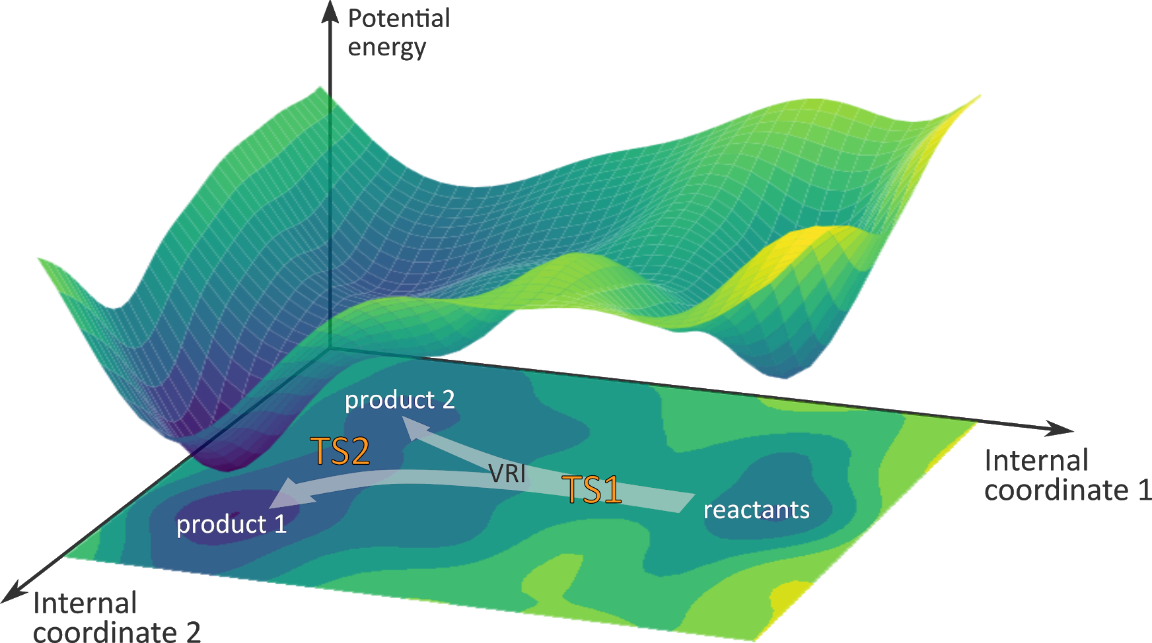
\includegraphics[width=1.0\textwidth]{FES1}
	\caption{Schematic representation of the potential energy surface and the stationary points.}
	\label{fig:FES1}
\end{figure}

The geometrical optimization of reactants and products consists in a minimization of the energy along the nuclear coordinates. Often the starting point is the experimental structure which can be obtained from diffraction data. In the most used codes several minimization methods are implemented, each characterized by a different computational cost and robustness, such as steepest descent, conjugated gradient or simulated annealing. The algorithms will find local minima, and do not guarantee that the system will be in a global minimum, therefore the minimizations must start from a sufficiently good guess. 
The search for transition states is far from trivial and often requires an iterative procedure involving different methods and requiring a good knowledge about the system and chemical process under study. In the calculations performed in this thesis, we often start from an equilibrium structure and as a first guess, we adapt the bond lengths and angles to be close to the transition state with a molecular editor such as Zeobuilder \cite{Verstraelen2008}. These bond lengths are then fixed, and the rest of the structure is reoptimized. The Hessian of this partly optimized structure needs to be then computed, and the vibrational modes analyzed, to check which (if any) negative frequency corresponds to the transition state. The system can be optimized again without the constraint using an improved dimer method along a selected eigenvector \cite{Heyden2005} which is followed by the optimization with a quasi-Newton method \cite{Press1989}. In some difficult cases, the TS search can be initiated on simpler cluster models and optimized in a code in which methods are usually implemented to directly find the TS structure. This way, a first guess of the TS geometry might be obtained and further transferred to the periodic model. In both transition states and minima, if there are superfluous negative frequencies, these need to be removed. Often, it is sufficient to minimize the energy along that vibrational mode. Single point energy calculations can be performed for different values of the displacement along that mode, and the lowest point in energy can be used as starting point for a subsequent minimization of all the coordinates.

\subsubsection*{Cell optimization}
In the case of periodic systems, not only the structure, but also the unit cell needs to be optimized. This is not trivial, as when using a finite plane wave basis set the number of plane waves depends on the volume of the unit cell. If the volume changes during the optimization, artificial forces which go under the name of Pulay stress can arise. This would require many iterations to optimize the volume. In this thesis, another approach was used \cite{Vanpoucke2015} which relies on an equation of state fit. For a given volume, for instance taken from experimental data, the unit cell is optimized. Then a set of equally spaced different volumes is defined and for each of these points the geometry and unit cell parameters are optimized. This way it is possible to construct an energy-volume curve, which for a rigid system can be fitted with a Birch-Murnaghan equation of state, allowing to extract the volume $V_0$ which corresponds to the minimum electronic energy $E_{0}$. 
\[
E(V) = E_{0} + 
\dfrac{9V_{0}B_{0}}{16}
\left\lbrace 
\left[\left(\dfrac{V_{0}}{V}\right)^{\frac{2}{3}} - 1\right]^{3} B'_{0} +
\left[\left(\dfrac{V_{0}}{V}\right)^{\frac{2}{3}} - 1\right]^{2}
\left[6 - 4\left(\dfrac{V_{0}}{V}\right)^{\frac{2}{3}}\right]
\right\rbrace
\]
Where $B_0$ and $B'_{0}$ are the bulk modulus and its derivative. A new structure is then generated at this given volume and coordinates and unit cell parameters are optimized again.

\subsection*{Molecular vibrations}
As seen in the previous paragraph, for many purposes in this thesis we need to calculate the second order derivatives (Hessian matrix) of the PES, which are associated to molecular vibrations. First of all, the Hessian gives us information about the curvature of the surface and the nature of the stationary points encountered during the minimization. The second order derivatives are obtained by displacing the atoms in the three directions and calculating the energies, then the Hessian is diagonalized to determine the eigenvectors that correspond to the vibrational motions. 
From the Hessian we can calculate the vibrational frequencies, which open the door to a lot more information on the system than a single point calculation. Single point calculations are performed at 0 K, but even at this temperature nuclei vibrate around their equilibrium positions, and this movements are responsible for the vibrational entropy. We can approximate these motions with those of harmonic oscillators, by using the vibrational frequencies constructed from the Hessian. These frequencies can then be used to estimate the value of the vibrational entropy at finite temperatures, as will be explained later. In the calculations performed in this thesis, due to computational limits, a partial Hessian approach was used when dealing with reactions, as implemented in the TAMkin toolkit \cite{Ghysels2010}. The quantity that needs to be derived from these calculations is the change in free energy, which mainly depends on the parts of the system that change during the reaction, in the case of a heterogeneous catalyst the active site and the adsorbed reactants. Therefore, restricting the entropy calculations only to this part of the system is a good approximation that allows to decrease enormously the computational cost \cite{Ghysels2007}. This approach has been used in the calculation of the free energy barriers for the Fischer esterification on UiO-66 (\textbf{PAPER I}), where the atoms taken into account were the adsorbed reactants and four atoms of the active sites in their immediate proximity, as displayed in Figure \ref{fig:PHVA}.

\begin{figure}[!htbp]
	\centering
 	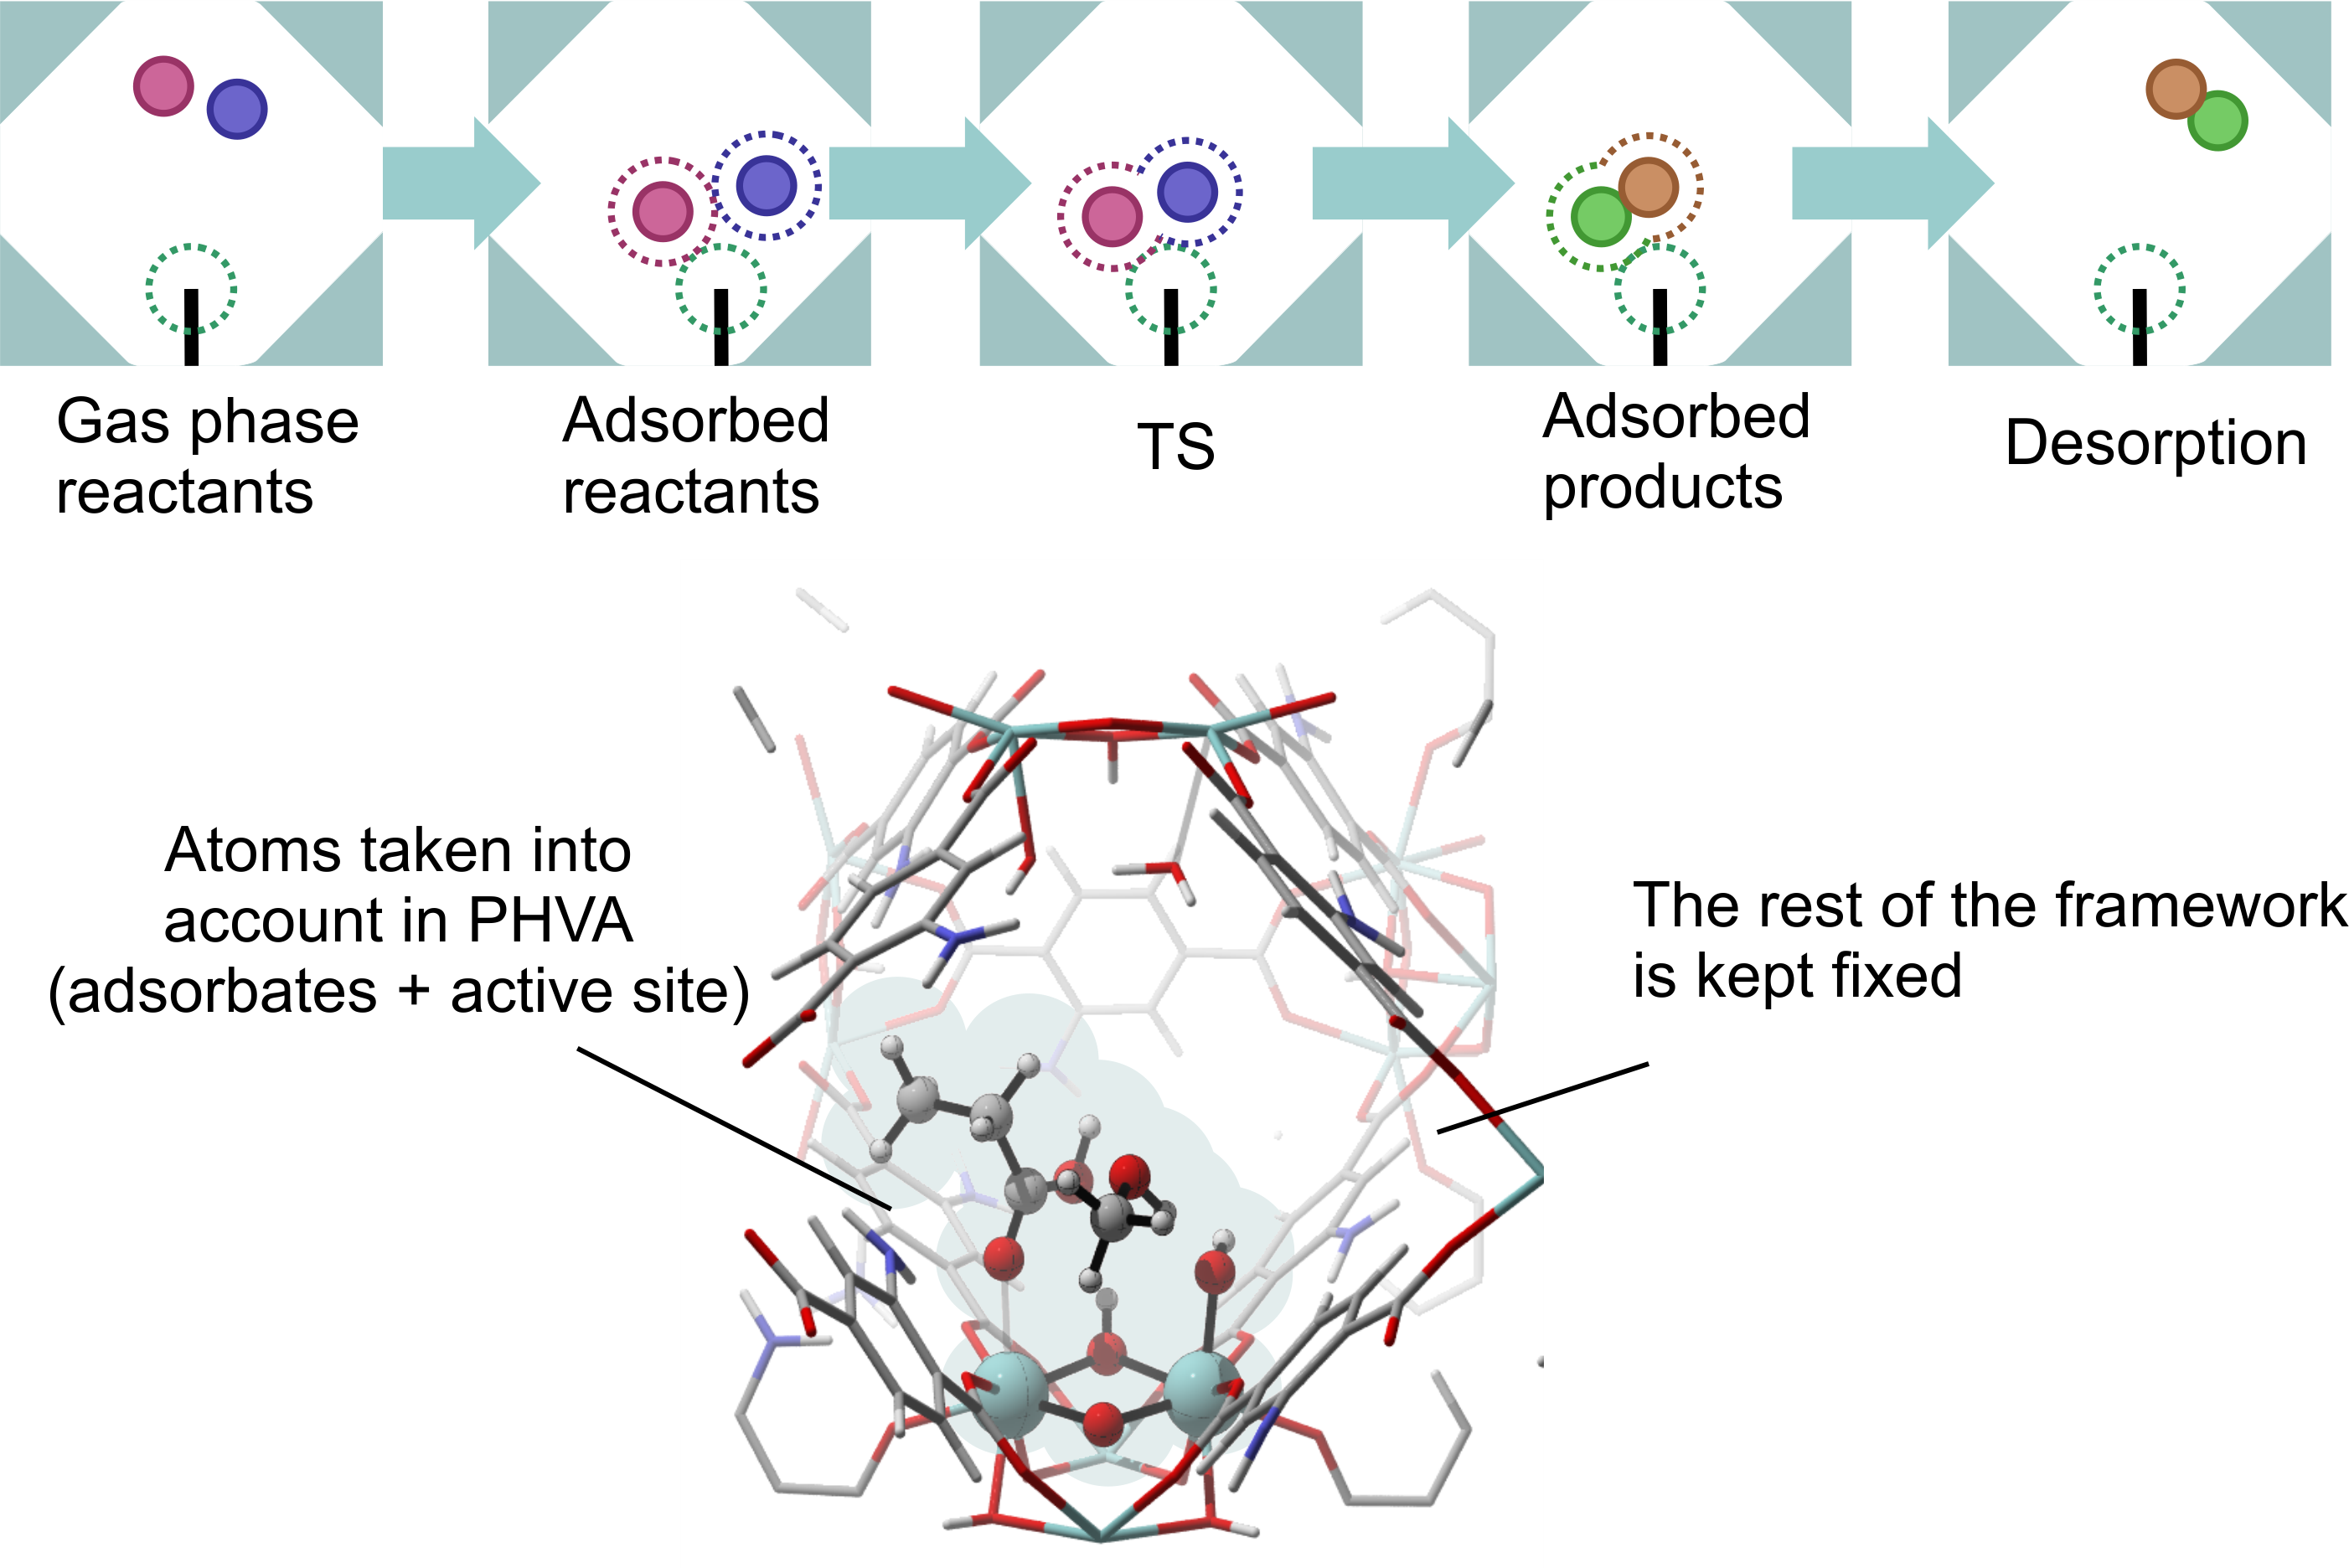
\includegraphics[width=1.0\textwidth]{PHVA}
	\caption{representation of the atoms taken into account in the PHVA approach. Top: a schematic representation of a reactive process in nanoporous material, bottom: a snapshot from the static calculations where the atoms of the active site and the adsorbates are highlighted}
 \label{fig:PHVA}
\end{figure}

\section{Free energy}
The central thermodynamic quantity that determines the outcome of a reaction is the free energy change associated to the process. In general, a chemical system will undergo changes in a direction that minimizes its free energy, until an equilibrium is reached. Knowing the difference in free energy between reactants and products allows us to know the equilibrium constant for a given reaction. The Gibbs Free energy can be decomposed in an enthalpic and an entropic contribution, that can be evaluated from the simulations knowing the molecular partition functions. Initially, the total internal energy $U$ has to be obtained from the electronic energy $\varepsilon_0$, the zero-point vibrational energy $E_{ZPE}$ and the molecular partition function $Q$ at constant number of particles $n$ and volume $V$:
\[
U = U_{0} + R T^{2}\left(\frac{\partial \ln Q}{\partial T}\right)_{n,V}
\]
\[ U_{0} = \varepsilon_{0} + E_{ZPE} \]
Where $R$ is the gas constant, equal to the product $N_{A}\cdot k_{B}$ between Avogadro's number and Boltzmann constant. The molecular partition function $Q$ can be split in its translational, rotational, and vibrational components:
\[
Q = Q_{trans}Q_{rot, ext}Q_{vib}
\]
The enthalpy $H$ corresponds to the total energy plus the work associated to the change in volume.
\[
H = U + p_{0}V
\] 
%H = U + p_{0}V = U + R T
The entropy $S$ can be directly obtained from the partition function:
\[
S = R \ln Q + RT \left(\frac{\partial \ln Q}{\partial
T}\right)_{n,V}
\]
Finally, the Gibbs free energy $G$ will be:
\[
G = H - TS = U_{0} + p_{0}V - RT\ln Q
\]
Where in the case of non-interacting particles $p_{0}V = RT$ following the ideal gas law. 

\subsection*{Equilibrium}
As explained above, there is a tight connection between free energy and equilibrium concentrations in chemical reactions. As an example, an equilibrium which is of outmost importance in chemistry is the acidic dissociation of species in aqueous solution:
\[
\ce{HA + H2O <=> A- + H3O+}
\]
The acidic dissociation constant ($K_a$)  is an important equilibrium constant in chemistry and is equal to the ratio between the concentration of products and reactants when the reaction reaches the equilibrium. It is often reported with its negative decimal logarithm as $pK_a$.
\[
K_a=\dfrac{\ce{[A- ][H+ ]}}{\ce{[HA]}} 
\]
The equilibrium constant is equal to the Gibbs free energy change from reactants to products.
\[
\Delta G = RT \ln K_a
\]
\[
pK_a = \dfrac{\ln 10}{RT} \Delta G
\]

\subsection*{Transition state theory}
A chemical reaction is a process that through rearrangement of the atoms transforms one stable state into another. Every elementary reaction can be represented as a minimum energy path connecting two minima along the potential energy surface. Furthermore, along this reaction path the existence of a saddle can be postulated, which is the highest point in energy that needs to be crossed to go to the product state. 
The saddle point is typically called transition state or activated complex and it is the basis for the transition state theory developed by Eyring in the 1930’s, one of the most successful chemical theories which allows to explain reaction rates of elementary chemical reactions. The assumption of the theory is that there is a quasi-equilibrium between reactants and activated complex, and the rate constant can be obtained by the size of the energy barrier and by the frequency at which the system can cross the barrier. This is possible because the barrier acts as a bottleneck in the reaction, its crossing is a rare event and all the kinetics depends only on it. For a unimolecular reaction, the rate constant can be derived from the partition functions of reactant, transition state and their energy difference:
\[
k(T) = \dfrac{{k_B T}}{h}
\dfrac{{q_{TS,\ddagger}}}{{q_R}} e^{- \frac{\Delta E^{\ddagger}}{k_B T}}
\]
Where $k_B$ is the Boltzmann constant, $h$ is the Planck constant, $q_R$  and  $q_{TS,\ddagger}$ are the molecular partition functions of reactants and activated complex for all coordinates except the reaction coordinate, evaluated from the zero-point vibrational level. 
\[
q_{vib,i} = \prod_{i=1}^{N_{dof}} \dfrac{1}{1 - e^{- \frac{h \nu_{i}}{k_B T}}}
\]
Where $N_dof$ are the number of vibrational degrees of freedom of the system. The energy difference $\Delta E^{\ddagger}$ includes electronic energy and zero-point vibrational energy difference at 0 K:
\[
\Delta E^{\ddagger} = E_{0}^{TS} - E_{0}^{R} + \Delta E_{0,vib}
\]
\[
\Delta E_{0,vib} = \sum_{i=0}^{N_{dof}-1} \frac{h \nu_{i}^{TS,\ddagger}}{2}
- \sum_{i=0}^{N_{dof}} \frac{h \nu_{i}^{R}}{2}
\]
This theory has some limitations, and may fail in the case of labile intermediates, when nuclei deviate from a classical behavior, or at high temperatures. For a given reaction, in fact, there will be many paths characterized by different barriers, and at low temperature only the lowest one will be likely to be crossed. When the kinetic energy is high enough, many other paths will be activated. The transition state will occupy a larger region of the PES, and it will not be possible to derive entropy from the vibrational partition functions.

\section{Exploring the free energy surface}
Static calculations, where molecular vibrations are approximated using harmonic oscillators, can fail to give an accurate representation of the entropy when there is a high configurational freedom. When the PES is flat with respect to $k_B T$, the system at equilibrium can evolve in a larger region of the PES and move along more than one minimum. In this case, vibrational frequencies are anharmonic and it is not possible to represent the system by approximating around one single minimum. Therefore, static calculations are not always sufficient in describing the system at operating conditions. In this view, molecular dynamics (MD) techniques, which follow the time evolution of the system, can resolve this shortcoming. 

\subsection*{Ab initio Molecular Dynamics}
From MD simulations, thermodynamic properties such as free energy can be obtained taking into account a whole region of the PES instead of a single point. This is based on the ergodic theorem, that states that the time average of equilibrium properties is equal to the ensemble average, in the limit of a sufficient long simulation. MD simulations are based on solving Newton’s equations of motion:
\[
M_i \ddot{\mathbf{R}}_i = \mathbf{F}_i = - \nabla_i V
\]
where $M_i$ and $\mathbf{R}_i$ are the mass of a given nucleus and its coordinates, $\mathbf{F}_i$ the forces that act on it, which correspond to the gradient $\nabla_i V$ of the PES. There are many ways to calculate these quantities and to integrate the equations of motion, and at present time, chemists and physicists can choose between a plethora of MD techniques which span a whole range of complexity, accuracy and computational cost. 
In the calculations performed in this thesis, potential energy and forces on the PES are calculated from first principles by means of DFT to account for the full dynamic behavior of the material by ab initio molecular dynamics (AIMD). The calculation of electronic properties which define the PES is decoupled from the propagation of nuclear motions, in a method called Born-Oppenheimer Molecular Dynamics (BOMD). Other famous AIMD methods, which differ by how the calculations of electronic potential and the equation of motion are combined, are the Car-Parrinello MD (CPMD)\cite{Car1985}, where a fictitious electronic kinetic energy is added to the lagrangian, or the Ehrenfest MD, based on the namesake theorem \cite{Ehrenfest1927, Marx2009}. The first MD calculations were performed in the microcanonical (NVE) ensemble, where total energy, number of particles and volume are fixed. However, in experiments it is often the temperature that is fixed, not the energy. In general, the choice of the ensemble depends on the thermodynamic quantities that need to be determined. Nowadays there are many thermodynamic ensembles in which the simulation can be performed. The most convenient for a comparison with experiments are the canonical (NVT), with fixed number of molecules, volume and temperature, or the isothermal-isobaric (NpT), with fixed number of molecules and temperature, but where the volume can fluctuate. In order to have a fixed average temperature, some control of the kinetic energy of the atoms is needed. Various thermostats, which differ by speed and robustness, are implemented in every MD code. In this thesis, Nose’-Hoover thermostat was used, where the system is connected to a heat bath. The pressure is also controlled in simulations by means of a barostat. The most commonly used is the one developed by Martyna, Tobias, and Klein (MTK)\cite{Martyna1994}.

\subsubsection*{Towards modeling at operating conditions}
With the growth in computational time, the new challenge is constituted by modeling the system at operating conditions. Many chemical reactions, especially when performed at mild conditions, involve the presence of a solvent. In order to move closer to modeling the system at operating conditions, the solvent in the pores can also be taken into account. This adds a lot of degrees of freedom to the system, and for this reason often an implicit description of the solvent is done, such as in the Periodic Continuum Model (PCM). In the case of the work in this thesis, however, it is necessary to fully model the solvent molecules, as they are actively involved in proton transfers. 
To do so, the number of solvent molecules that can fit in the unit cell needs to be estimated. Monte Carlo method (MC) is an alternative approach to MD to explore the PES for complex systems. It was initially developed for the calculation of multidimensional integrals and is nowadays largely used in chemistry, especially when dealing with adsorption. In the framework of this thesis, it has been applied in the Gran Canonical ensemble (fixed chemical potential, volume and temperature) to determine the number of solvent molecules that could fill the pores of the material at standard conditions.

\subsection*{Enhanced MD methods}
MD simulations can offer valuable insights into the behaviour of a chemical system at equilibrium conditions. From these simulations, many properties can be extracted, such as equilibrium geometries, vibrational spectra, diffusion coefficients, structural parameters etc. Configurations associated to higher (or lower) values of potential energies will be sampled for shorter (or longer) times, and in principle, if a certain process is sufficiently sampled, based on the ergodic theorem we can know its equilibrium constant, and in turn the free energy barrier associated to it. However, chemical reactions, where bonds are broken and formed, are generally rare events that will not be sampled with a regular exploration of the PES. If the barrier is high compared to the $k_{B}T$, the probability that such event would spontaneously occur during the simulation time is practically none. For this reason, different enhanced sampling techniques have been developed to enhance the sampling of certain regions of the PES. 


\subsubsection*{Choice of collective variable}
The PES is a highly dimensional surface, defined by the positions of all atoms in the system. However, often a reactive process can be described by few important coordinates called ``collective variables'' (CV), which are projections of the high dimensional space. In fact, what can be considered a chemical configuration is an ensemble of microstates that are different in terms of absolute coordinates of each atom, but all contribute to the same macrostate.
In the simplest case, a single CV can represent the reaction coordinate for the process.

The choice of the right collective variable is crucial to describe the correct process. 
\td{what are the main choices, distances, CN, angles}


\subsubsection*{Metadynamics}



\subsubsection*{Umbrella sampling}



\clearpage{\pagestyle{empty}\cleardoublepage}

%%%%%%%%%%%%%%%%%%%%%%%%%%%%%%%%%%%%%

%\subsection*{\textit{Ab initio} molecular dynamics}
%In order to sample conformational freedom and adsorption of substrates at true operating conditions usage of a dynamical approach is required, in which effects of temperature, pressure and flexibility of the material can be taken into account. In molecular dynamics (MD) simulations the time--dependent motion of a system is defined at the molecular level by solving Newton's equation. Within the framework of this thesis various \textit{ab initio} MD simulations were performed based on a periodic DFT description including Grimme D3 dispersion corrections \cite{Grimme2010}. In the MD simulations the temperature and pressure were controlled by a chain of five Nos\'e--Hoover thermostats and by a Martyna--Tobias--Klein (MTK) barostat, respectively \cite{Frenkel2002, Martyna1994}. Such simulations can be performed in different thermodynamics ensembles and the most commonly applied are the canonical ensemble (NVT) and the isobaric--isothermal (NPT) ensemble. In what follows, we will illustrate by means of three case studies the pros and cons of various simulations techniques to study adsorption.
%\npar
%To show the complementarity of various methods to describe adsorption an example is given from \textbf{Paper X}. The position of adsorbed dimethyl methylphosphonate (DMMP) as a case study model for the infamous 'nerve agent' group of alkyl phosphonate compounds was investigated in the defective UiO--66(\ce{NH2}). The insight in the adsorption of the DMMP molecule in the defective amino--functionalized material was obtain by periodic static and dynamic DFT calculations. Both types of simulations revealed two possible adsorption sites. The adsorption can either occur in an adjacent position to a linker defect in the octahedral cage or directly in the position of a missing linker as shown in Figure \ref{fig:DMMP}. In the first case, long range interactions between the amino groups and DMMP appear to be important stabilizing the adsorption position, while in the second case, the molecule interacts closely with water molecules and hydroxyl groups capping the defect sites on the brick. For both sites the statically calculated electronic adsorption energy is of about 100 kJ/mol. To verify the mobility of the adsorbate in the framework the MD simulations at 300 K were performed starting from both adsorption positions. During 20 ps of simulations the DMMP molecule maintained the initial adsorbed position, which further underlines its strong adsorption on both sites. The NPT simulations allowed a comprehensive study of the synergies that point towards many confined interactions between the adsorbed molecule and the UiO--66(\ce{NH2}) framework \cite{Stassen2016}.
%
%\begin{figure}[!h]
%	\centering
%	\includegraphics[width=1.0\textwidth]{DMMP}
%	\caption{Snapshots of two possible adsorption configurations of the DMMP
%	molecule in the pores of UiO--66(\ce{NH2}). Right: top panel
%	presents an adjacent position of DMMP to a
%linker defect in the octahedral cage; bottom panel shows the
%	adsorption of DMMP in the position of a missing linker.}
%	\label{fig:DMMP}
%\end{figure}
%\npar
%\newpage
%A multilevel modeling approach was
%applied in \textbf{Paper VIII} to study the adsorption of methanol in
%defective UiO--66. The estimation of loading of guest species within the pores
%of nanoporous materials has drawn a lot of attention, for which typically, grand
%canonical Monte Carlo (GCMC) simulations have been applied. These simulations
%are performed with empirical force field models that do not describe the
%electronic structure of the host--guest interactions, however, information
%about the most plausible adsorption sites can be obtained. In this respect, the
%description of methanol solvent introduced in the pores was done by GCMC
%applying a universal force field, followed by a series of MD simulations using
%the PBE functional at NPT and NVT ensembles. The D3 corrections were included
%throughout geometry optimizations of molecular dynamics runs. In the simulations the appearance of various networks between methanol and water on the active
%sites was detected. The configurations range from single closed loops of
%hydrogen bonded methanol and water molecules to closed loops and open
%methanol chains including up to 5--6 molecules (Figure
%\ref{fig:methanol}). Interestingly, the structure of bulk methanol shows
%some correspondence with the structure in a confined environment
%\cite{Caratelli2017a}.
%
%\begin{figure}[!h]
%	\centering
%	\includegraphics[width=1.0\textwidth]{methanol}
%	\caption[Schematic representation of a pore in UiO--66. Left: periodic
%	lattice; right: the pore where the missing linker defect is located, with
%	included guest molecules. The active sites A and B are indicated
%	on the left. Bottom: Ring configurations observed at sites A and B which arise
%	from the interaction between the Zr--bonded hydroxyl groups and water and the solvent
%molecules.]{Schematic representation of
%a pore in UiO--66. Left: periodic lattice; right: the pore where the missing linker defect is located, with
%	included guest molecules. The active sites A and B are indicated
%	on the left. Bottom: Ring configurations observed at sites A and B which arise
%	from the interaction between the Zr--bonded hydroxyl groups and water and the solvent
%molecules. Adapted from Ref. \cite{Caratelli2017a}.}
%	\label{fig:methanol}
%\end{figure}
%\npar
%\clearpage
%Another advanced periodic multilevel modeling approach was used to follow the
%adsorption of pentene in H--ZSM--5 in \textbf{Paper VI}. Initially, a series of
%\textit{ab initio} MD simulations was performed at 323 K on 1--pentene, 2--
%pentene, 2--pentoxide and 3--pentoxide $\pi$--complexes to gain insight into the
%mobility of the various adsorbed species (Figure
%\ref{fig:pentene}). Preliminary MD runs of about 10 ps
%were executed, in which the physisorbed pentene molecule was oriented in the
%center of the straight 10--membered ring cavity at about 4 \AA\ from the acid
%site. The diffusion of the 2--pentene from an unbiased initial position, in
%which the adsorbate only interacts with the framework of the zeolite quickly
%evolves towards the acid site to form the $\pi$--complex. The preferential
%orientation of the 2--pentene molecule is in the intersection of the two pores,
%which corresponds to the methyl tail directed in the zig--zag channel near the
%Br\o{}nsted acid site and the longer ethyl tail in the straight cavity (Figure
%\ref{fig:pentene}, b).
%These initial MD runs were used to select configurations for a subsequent set of extensive MD simulations of 100 ps. For both 1-- and 2--pentene the shortest \ce{C-H} distance remains on average
%of about 2 \AA, pointing that the \ce{$\pi$-H} interaction is in place
%throughout the simulation. A similar position analysis was made for the alkoxides
%indicating that these complexes are also stable during the simulation with
%average \ce{C-O} distances of about 1.6 \AA. In the MD simulations at 323 K we
%did not observe the formation of carbenium ions.
% 
%\begin{figure}[!h]
%	\centering
%	\includegraphics[width=1.0\textwidth]{pentene}
%	\caption[MD snapshots of (a) 1--pentene $\pi$--complex, (b) 2--pentene
%	$\pi$--complex, (c) chemisorbed 2--alkoxide and (d) chemisorbed 3--alkoxide in
%	H--ZSM--5 at 323 K, seen in the direction of the straight channel (camera
%	viewpoint). The snapshots correspond to geometries which are most frequently visited during MD runs of
%100 ps at 323 K.]{MD snapshots of (a) 1--pentene $\pi$--complex, (b) 2--pentene
%	$\pi$--complex, (c) chemisorbed 2--alkoxide and (d) chemisorbed 3--alkoxide in
%	H--ZSM--5 at 323 K, seen in the direction of the straight channel (camera
%	viewpoint). The snapshots correspond to geometries which are most frequently visited during MD runs of
%100 ps at 323 K. Reproduced from Ref. \cite{Hajek2016} with permission of
%Elsevier, copyright 2016.}
%	\label{fig:pentene}
%\end{figure}
%\clearpage
%Subsequently, based on the
%probability distribution plotted in Figure \ref{fig:probability} the adsorption
%positions corresponding to the most frequently visited structures during the MD runs were determined to optimize these geometries statically. Thereafter, information about the adsorption enthalpies was obtained from the frequency calculations and the influence of finite temperature effects on the adsorption enthalpies was assessed.
%The plotted probability distributions for the distances of the various adsorbed
%species in H--ZSM--5 show an asymmetric behavior for the $\pi$--complexes
%towards higher \ce{C-H} distances.
%The adsorption enthalpy of physisorbed species of 1-- and 2--pentene is heavily
%allied with the \ce{C-H} distance.
%The broad probability distribution for these two molecules illustrates that the
%average ensemble over the MD simulations results in enthalpy of adsorption which
%coincides to \ce{C-H} distances larger than 2 \AA.
%This contrasts with the static calculations, in which only one minimum on the
%potential energy surface is considered excluding configurations with slightly
%larger distances which are detected in the MD simulations. Summarizing, the
%dynamically averaged values of the adsorption enthalpies give systematically
%lower values for the $\pi$--complexes and slightly higher values for the
%alkoxides adsorption enthalpic energies. The position of the double bond does not significantly
%affect the enthalpy of formation of the $\pi$--complexes which was also observed
%by Bhan \textit{et al.} \cite{Bhan2003}. Furthermore, by taking into account
%finite temperature effects, the $\pi$--complexes are almost equally stable as the
%alkoxide species \cite{Hajek2016}.
%
%\begin{figure}[!h]
%	\centering
%	\includegraphics[width=1.0\textwidth]{probability}
%	\caption[Probability distributions of observing some distances in molecular
%	dynamics simulations of $\pi$--complexes and alkoxides in H--ZSM--5 throughout
%	the final 60 ps simulation time.]{Probability distributions of observing some distances in molecular
%	dynamics simulations of $\pi$--complexes and alkoxides in H--ZSM--5 throughout
%	the final 60 ps simulation time \cite{Hajek2016}. Reproduced with
%	permission of Elsevier, copyright 2016.}
%	\label{fig:probability}
%\end{figure}
%
%
%\subsection*{Enhanced sampling MD methods}
%In principle, MD simulations allow access to free energy profiles of chemical reactions, however, due to the broad range of characteristic time scales related to a molecular system this task is far from trivial \cite{ Fleurat2005}. Chemical reactions are most of the time rare events and the barrier from a reactant to a product state is usually too high, which gives rather low probabilities of happening during a regular MD run of a few ps.  This limitation can be overcome by using different available advanced molecular dynamics techniques. Currently, a whole plethora of these enhanced sampling methods  is available, which allow exploring low probability regions of the free energy surface \cite{ Laio2002,  Sutto2012, Carter1989, Darve2001, Jarzynski1997,  Rosso2002, Gullingsrud1999}. Detailed reviews on the advanced molecular dynamics simulations are given in the work of Valsson \textit{et al.}\cite{Valsson2016} and references therein. The enhanced sampling MD techniques have only recently been successfully applied in the field of heterogeneous catalysis to study chemical reactions at true operating conditions of temperature and pressure \cite{DeWispelaere2016, DeWispelaere2015, VanSpeybroeck2014, Cnudde2017, Haigis2015, Bucko2011}. An overview of the recent advances in computational techniques for nanoporous materials can be found in Ref.\cite{Evans2017, Fraux2017}. In general, two classes of these methods can be distinguished. In the first class, dynamics techniques enhance the sampling of all degrees of freedom. The Replica Exchange (RE) \cite{Sugita1999} and Transition Path Sampling (TPS)\cite{Dellago2006} methods are very useful to discover new reaction mechanisms without the prior knowledge or definition of transition states. These methods applied in the field of porous materials have the ability to predict selectivity for various products of zeolite--catalyzed reactions, as was indicated by Bu\u{c}ko \textit{et al.}\cite{Bucko2009}. 
%In the second class of advanced dynamics methods, techniques are defined in which the sampling of low probability regions is enhanced along certain coordinates. The most common are Umbrella Sampling (US)\cite{Patey1975, Torrie1977} and Metadynamics (MTD) \cite{Laio2002}. The latter coordinates are commonly referred to as collective variables (CV) which may be internal coordinates such as bond lengths, bond angles or more complex variables like coordination numbers \cite{Rohrdanz2013}. The free energy methods considered in this work are schematically represented in Figure \ref{fig:dynamic}. 
%
%\subsubsection*{Metadynamics}
%MTD first introduced by Laio and co--workers \cite{Laio2002}, is a popular method to accelerate the occurrence of reactions in which a bias potential by means of Gaussian hills is added to the potential energy surface. The bias potential is updated on--the--fly, artificially increasing the potential energy of the already visited states. In such a fashion, states other than the local minima are sampled in an MTD approach. There exist various algorithms to update the potential energy surface, most notably is the variational approach. When all states become equally probable under the combined action of the potential energy surface and the bias potential, the free energy is equivalent to the inverse bias potential. The method serves as an excellent tool to scan the configuration space in the direction of the CV for possible minima and has recently been applied successfully in various zeolite catalysis studies \cite{DeWispelaere2015, DeWispelaere2016}.
%
%\begin{figure}[!h]
%	\centering
%	\includegraphics[width=1.0\textwidth]{dynamic}
%	\caption[Schematic representation of the free energy methods considered in this work. Each panel represents a different free energy method. Within
%each panel, the top figure shows the simulation result and the bottom figure concerns the estimated free energy profile. The color coding is black for
%the unknown free energy, green for the simulation results and the estimated free
%energy, and purple for the sampling methods. Below the method panel,a possible
%2--D representation of the given reaction on the two active sites as obtained using
%advanced dynamic techniques, indicating the three critical points on the potential energy surface.]{Schematic representation of the free energy methods considered in
%	this work. Each panel represents a different free energy method. Within each panel, the top figure shows the simulation result and the bottom figure concerns the estimated free energy profile. The color coding is black for
%the unknown free energy, green for the simulation results and the estimated free
%energy, and purple for the sampling methods. Below the method panel,a possible
%2--D representation of the given reaction on the two active sites as obtained using
%advanced dynamic techniques, indicating the three critical points on the
%potential energy surface. Adapted from Ref.\cite{Demuynck2017} and \cite{Rogge2017}.}
%	\label{fig:dynamic}
%\end{figure}
%
%
%\subsubsection*{Umbrella sampling}
%In US an external potential is added to the true Hamiltonian to improve the sampling of low probability regions along defined coordinates of the system. By performing various US simulations, targeting different regions of the CV, the entire range of interest in terms of the CV can be sampled. A free energy profile can be estimated employing a scheme connecting the local information from the various simulations, such as the weighted histogram analysis method or multistate Bennett acceptance ratio \cite{Kumar1992, Patey1975, Torrie1977}. Being highly parallelizable US is a very efficient sampling method. Nevertheless, prior knowledge is required both in terms of an accurate CVs and a descent estimate of the various stable states.
%
%
%\subsubsection*{Choice of CV}
%The success of the MTD and US methods critically relies on a decent
%choice of the CVs which enable to lead the
%system to parts of interest on the free energy surface. The suitable choice is
%not evident and requires a good insight about a studied
%reaction \cite{Rohrdanz2013}. When simulating complex chemical transformations,
%the use of non geometric parameters by means of coordination numbers are especially advisable to describe CV. The coordination number CN used in the simulation is formally
%defined as: 
%\[
%\mathrm{CN} =\sum_{i,j}\frac{1-(r_{ij}/r_0 )^{nn}}{1-(r_{ij}/r_0 )^{nd}}
%\] 
%\\
%where the sum runs over two sets of atoms ${i}$ and ${j}$, $r_{ij}$ defines the
%distance between atoms i and j and $r_0$ is a reference distance. The parameters
%$nn$ and $nd$ are usually set to 6 and 12, respectively. 
%\npar
%The definition of CV in terms of two coordination numbers was used in
%\textbf{Paper VI} to study the formation of the activated transitions on the
%reaction path on the formation of 2--pentoxide from physisorbed 1--pentene and
%2--pentene and that of 3--pentoxide from physisorbed 2--pentene. The results
%from MTD simulations to sample the possible occurrence of carbenium ions in the
%reaction paths from $\pi$--complexes to alkoxides are shown in Figure
%\ref{fig:2_3_pentoxide_FES}. To describe the proton transfer from the zeolite framework to the pentene molecule, the combined coordination number of
%\ce{O-H} bond cleavage and \ce{C-H} bond formation was defined as CV1:
%\ce{CN(O-H)-CN(C_1-H)}.
%The formation of the \ce{C-O} bond between the resulting pentyl carbenium ion
%and the zeolite framework was investigated with the second CV2 as \ce{CN(C_2-O)}
%as displayed in Figure \ref{fig:2_3_pentoxide_FES}, top.
%The carried out MTD simulations resulted in 2--D free energy surface. 
%In the case where more than one CV is applied to describe the process, it is
%necessary to project the resulting free energy surface of the multidimensional
%simulations into a lower dimensional coordinate \cite{DeWispelaere2015}. The
%lowest free energy path (LFEP) method proposed by Ensing \textit{et al.}
%\cite{Ensing2005} was successfully applied to obtained a 1--D profile. The
%lowest free energy paths describing the three transformations in 2--D and
%1--D energy surfaces are displayed in Figure \ref{fig:2_3_pentoxide_FES}.
%The existence of a metastable state between the $\pi$--complex and the pentoxide is evident and characterized as a pentene carbenium ion.
%
%\begin{figure}[!htp]
%	\centering
%	\includegraphics[width=0.95\textwidth]{2_3_pentoxide_FES}
%	\caption[Top: Schematic representation of the applied collective variables.
%	Left: 2--D free energy surface for the formation of 2--pentoxide from a
%	1--pentene $\pi$--complex (a) or 2--pentene $\pi$--complex (b) and for the formation
%	of 3--pentoxide from a 2--pentene $\pi$--complex (c). The lowest free energy paths
%	are displayed. A small well corresponding to the metastable carbenium ion can be observed in the bottom left corner.
%Right: corresponding 1--D free energy profile along the lowest free energy path
%for the two reactions.]{Top: Schematic representation of the applied collective variables.
%	Left: 2--D free energy surface for the formation of 2--pentoxide from a
%	1--pentene $\pi$--complex (a) or 2--pentene $\pi$--complex (b) and for the formation
%	of 3--pentoxide from a 2--pentene $\pi$--complex (c). The lowest free energy paths
%	are displayed. A small well corresponding to the metastable carbenium ion can be observed in the bottom left corner.
%Right: corresponding 1--D free energy profile along the lowest free energy path
%for the two reactions. Reprinted with permission from Ref.\cite{Hajek2016}.}
%	\label{fig:2_3_pentoxide_FES}
%\end{figure}
%\npar


%\newpage
%In summary the plethora of techniques presented in this Chapter, shows that
%nowadays a rich computational toolbox is available to study chemical reactions in zeolites and MOFs.
%At the onset of this PhD thesis, a lot of cluster based models were still used, 
%whereas today usage of periodic DFT based methods has become more common.  
%A very intriguing evolution within the time frame of this thesis, is the ability
%to simulate chemical reactions at operating conditions, using advanced MD
%methods. Finally the particular choice of methods is guided by the system at
%hand, computational resources and the phenomenon one wishes to describe.
%Regarding computational costs, it needs to be mentioned that first principle MD
%based methods are computationally very expensive and may not be regarded as the standard method to study any reaction at hand. 
%For information, to describe the same chemical transformation static simulations
%take approximately 20--25 nodedays and MD simulations around 150--200 nodedays
%(Machine specs: 2 x 10--core Intel E5--2660v3 (Haswell--EP @ 2.6 GHz)).
\clearpage{\pagestyle{empty}\cleardoublepage}
